\hypertarget{scope}{%
\section{Scope}\label{scope}}

This is the scope description.

There may be mutliple paragraphs.

Or even a list:

\begin{itemize}
\tightlist
\item
  wun
\item
  two
\item
  three
\end{itemize}

\hypertarget{scope-subsection}{%
\subsection{Scope Subsection}\label{scope-subsection}}

Sometimes authors even insert subsections into the scope.

\hypertarget{glossary}{%
\subsection{Glossary}\label{glossary}}

\begin{description}
\tightlist
\item[Term]
Words with special meaning
\item[Design\_Term]
Terms with meaning different from similar words in the natural language.
\end{description}

\hypertarget{references}{%
\section{References}\label{references}}

\begin{description}
\tightlist
\item[{[}REF-A{]}]
Reference A, Stockholm, 2022
\item[{[}REF-B{]}]
Reference B, Paris, 1821
\end{description}

\hypertarget{architecture}{%
\section{Architecture}\label{architecture}}

The top level plan in use for building the best software ever.

Blueprints may link to visuals like \ref{fig:blue-square} and link to
them.

\begin{figure}
\centering

\includegraphics[width=0.98\textwidth,height=0.98\textheight]{images/blue.png}
\caption{Blue Square}
\end{figure}

In some cases backward references to figures like \ref{fig:blue-square}
are in use.

It is not always possible to stop organizations from creating deeply
nested matrioshka like section trees.

Let us test how this passes the publication or rendering pipeline.

\hypertarget{why-not}{%
\subsection{Why Not?}\label{why-not}}

Second level heading results in a subsection under our regime.

\hypertarget{this-is-ok}{%
\subsubsection{This is OK}\label{this-is-ok}}

Third level results in subsubsection.

\hypertarget{is-this-really-useful}{%
\paragraph{Is this really useful?}\label{is-this-really-useful}}

Laying out a level four heading should end in a paragraph.

\hypertarget{until-the-cows-come-home}{%
\subparagraph{Until the Cows Come Home}\label{until-the-cows-come-home}}

Overengineering is so much fun.

This is not Funny for Anyone

Who knows where we are in the tree and if we evver see the light of the
sun again \ldots{}

\hypertarget{lists-maybe}{%
\subsection{Lists Maybe?}\label{lists-maybe}}

Unordered, nested, and tight?

\begin{itemize}
\tightlist
\item
  wun

  \begin{itemize}
  \tightlist
  \item
    wunder
  \end{itemize}
\item
  two
\item
  three

  \begin{itemize}
  \tightlist
  \item
    hree

    \begin{itemize}
    \tightlist
    \item
      ree

      \begin{itemize}
      \tightlist
      \item
        re

        \begin{itemize}
        \tightlist
        \item
          e
        \end{itemize}
      \end{itemize}
    \end{itemize}
  \end{itemize}
\item
  four
\end{itemize}

Ordered and tight:

\begin{enumerate}
\def\labelenumi{\arabic{enumi}.}
\tightlist
\item
  uno
\item
  due
\item
  tre
\end{enumerate}

And a fenced code block:

\begin{Shaded}
\begin{Highlighting}[]
\DataTypeTok{int}\NormalTok{ main}\OperatorTok{()\{\}}
\end{Highlighting}
\end{Shaded}

This is all we write about the architecture.

Wait, mermaids!

\begin{figure}
\centering
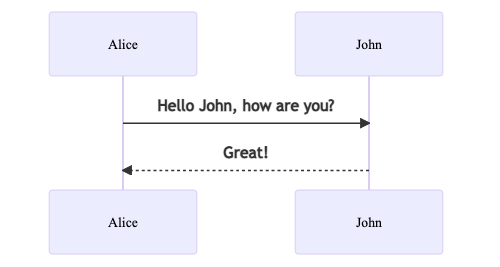
\includegraphics{images/alice-and-john.png}
\caption{Alice and John - Relationship as a Sequence}
\end{figure}

The auto-generated label should make the reference work like so:
\ref{fig:alice-and-john}. Does it?

\hypertarget{design}{%
\section{Design}\label{design}}

Now we really write down details.

Pictures with labels \ref{fig:green} to be injected:

\begin{figure}
\centering

\includegraphics[width=0.95\textwidth,height=0.33333in]{images/green.png}
\caption{Green Square Scaled as Rectangle}
\end{figure}

And, did it work?

\hypertarget{tables}{%
\subsection{Tables}\label{tables}}

A table:

\begin{longtable}[]{@{}lcr@{}}
\toprule()
Left & Middle & Right \\
\midrule()
\endhead
L & CC & R \\
l & Cc & R \\
L & cC & r \\
\bottomrule()
\end{longtable}

A caption \label{tab:sweet-and-lovely}

Some real paragraph of dense text representing deep thoughts about
appearance. Some real paragraph of dense text representing deep thoughts
about appearance. Some real paragraph of dense text representing deep
thoughts about appearance. Some real paragraph of dense text
representing deep thoughts about appearance. Some real paragraph of
dense text representing deep thoughts about appearance. Some real
paragraph of dense text representing deep thoughts about appearance.
Some real paragraph of dense text representing deep thoughts about
appearance.

A quote:

\begin{quote}
That's all folks.
\end{quote}

And final words.

\hypertarget{a-final-diagram}{%
\subsubsection{A Final Diagram}\label{a-final-diagram}}

Here is a final diagram:

\scale=0.95

\begin{figure}
\centering

\includegraphics{diagrams/squares-and-edges.png}
\caption{Squares and Edges}
\end{figure}

We can refer to the diagram (whuch will be scaled to 95\% of the page
width per \ref{fig:squares-and-edges} namely the default injected label.

Oh, \emph{cursive} and \textbf{bold} \ldots{} are easily indicated.

\hypertarget{abbreviations}{%
\section{Abbreviations}\label{abbreviations}}

\begin{description}
\tightlist
\item[ABC]
Indicator for an alphabet
\item[IO]
Input Output
\item[UI]
User Interface
\end{description}
